% !TEX root = ../main.tex
% linea de arriba: hace que los  compiladores compilen el documento  main.tex al tratar de compilar este documento
Desarrollo \cite{wikipedia1}

\begin{figure}[H]
  \centering
  \begin{subfigure}[b]{0.475\textwidth}
    \centering
        {
          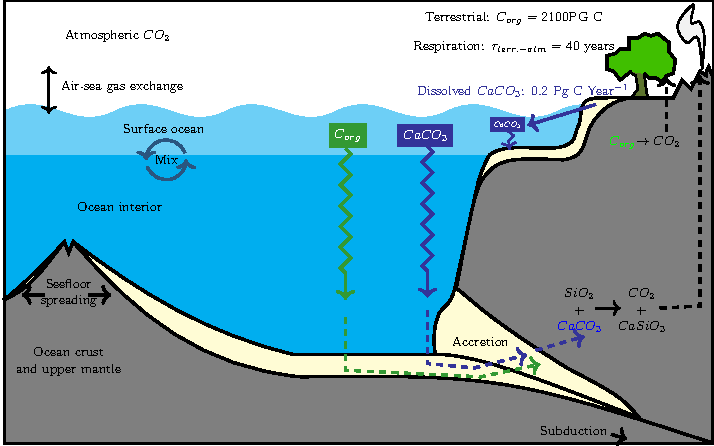
\includegraphics[width= 0.9\textwidth]{img/figura.pdf} % pdf
        }
        \caption{$t=1$}     
  \end{subfigure}
  \begin{subfigure}[b]{0.475\textwidth}
    \centering
        {
          \includestandalone[width=0.9\textwidth]{img/figura2} % tikz
        }     
        \caption{$t=2$}
  \end{subfigure}
\caption{Ejemplo de figura.}\label{fig: ejem}
\end{figure}

\begin{lstlisting}
for i = 1:3
  if i >= 5 && a ~= b       % literate programming replacement
    disp('cool');           % comment with some §\mcommentfont\LaTeX in it: $\mcommentfont\pi x^2$§
  end
  [:,ind] = max(vec);
  x_last = x(1,end) - 1;
  v(end);
  really really long really really long really really long really really long really really long line % blaaaaaaaa
  ylabel('Voltage (µV)');
end
\end{lstlisting}